\newread\syntheticgrpcfile%

\newcommand{\IfNonemptySyntheticGrpcFile}[3]{%
    \IfFileExists{#1}{%
        \openin\syntheticgrpcfile=#1
        \ifeof\syntheticgrpcfile%
            \closein\syntheticgrpcfile%
            #3%
        \else
            \closein\syntheticgrpcfile%
            #2%
        \fi
    }{%
        #3%
    }%
}

\newcommand{\SyntheticGrpcPlot}[3]{%
    \IfNonemptySyntheticGrpcFile{#3}{%
        \addplot+[#1]
        table [#2, col sep=comma] {#3};
    }{}%
}

\begin{figure}[!t]
    \centering

    \begin{subfigure}[b]{\linewidth}
        \begin{tikzpicture} [scale=0.875, transform shape]
        \begin{axis}
                [
                ylabel={Latency (us)},
                legend style={draw=none},
                ylabel={Latency(us)},
                xmin=0,
                ymin=0,
                ymax=2000,
                xmax=275,
                height=3.3cm,
                width=\linewidth,
                restrict x to domain*=0:5E9,
                restrict y to domain*=0:1E4,
                axis y line=left,
                axis x line=bottom,
                legend cell align=left,
                legend style={
                draw=none,
                font=\footnotesize,
                anchor=south,
                at={(0.5, 1.0)},
                legend columns=2,
                /tikz/every even column/.append style={column sep=0.8cm},
                },
                ]
            \addlegendimage{grpc_vanillaStyle, dotted, cLightPurple!80, mark=*}
            \addlegendentry{gRPC-POSIX-24}

            \addlegendimage{grpc_rakaiaStyle, dotted, cViolet!80, mark=*}
            \addlegendentry{grpc-\system-24}

            \addlegendimage{grpc_vanillaStyle}
            \addlegendentry{gRPC-POSIX-5,000}

            \addlegendimage{grpc_rakaiaStyle}
            \addlegendentry{grpc-\system-5,000}

            \SyntheticGrpcPlot{
                grpc_rakaiaStyle, line width=2pt, dotted, cViolet!70, mark=*,
                x filter/.code={
                    \IfStrEq{\thisrow{dist_config}}{exponential}{}{\def\pgfmathresult{}}
                }
            }{x expr=\thisrow{load_grpc-rakaia-go(QPS)} / 1000, y=latency_grpc-rakaia-go}{data/synthetic_grpc_24conn.csv}

            \SyntheticGrpcPlot{
                grpc_vanillaStyle, line width=2pt, dotted, cLightPurple!70, mark=*,
                x filter/.code={
                    \IfStrEq{\thisrow{dist_config}}{exponential}{}{\def\pgfmathresult{}}
                }
            }{x expr=\thisrow{load_grpc-go(QPS)} / 1000, y=latency_grpc-go}{data/synthetic_grpc_24conn.csv}

        \end{axis}
        \end{tikzpicture}
    \end{subfigure}

    \begin{subfigure}[b]{\linewidth}
        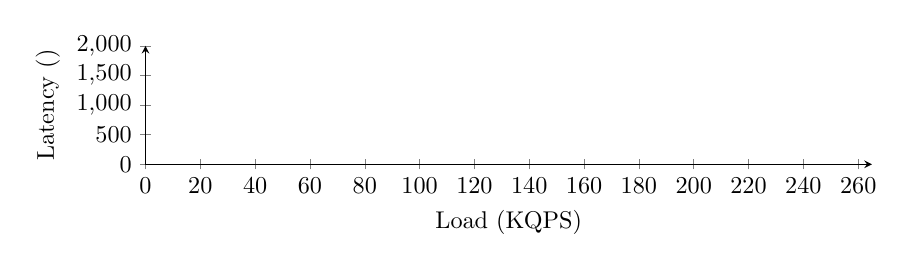
\begin{tikzpicture} [scale=0.875, transform shape]
            \begin{axis}
                [
                xlabel={Load (KQPS)},
                ylabel={Latency (\si{\micro\second})},
                legend style={draw=none},
                xmin=0,
                ymin=0,
                height=3.3cm,
                width=\linewidth,
                xmax=265,
                ymax=2000,
                enlarge y limits=false,
                restrict x to domain*=0:5E9,
                restrict y to domain*=0:1E4,
                axis y line=left,
                axis x line=bottom,
                legend cell align=left,
                legend style={
                draw=none,
                font=\footnotesize,
                anchor=south,
                at={(0.5, 1.1)},
                legend columns=2,
                /tikz/every even column/.append style={column sep=0.8cm},
                },
                ]

                \SyntheticGrpcPlot{
                    grpc_rakaiaStyle, line width=2pt,
                    x filter/.code={
                        \IfStrEq{\thisrow{dist_config}}{exponential}{}{\def\pgfmathresult{}}
                    }
                }{x expr=\thisrow{load_grpc-rakaia-go(QPS)} / 1000, y=latency_grpc-rakaia-go}{data/synthetic_grpc_5000conn.csv}

                \SyntheticGrpcPlot{
                    grpc_vanillaStyle, line width=2pt,
                    x filter/.code={
                        \IfStrEq{\thisrow{dist_config}}{exponential}{}{\def\pgfmathresult{}}
                    }
                }{x expr=\thisrow{load_grpc-go(QPS)} / 1000, y=latency_grpc-go}{data/synthetic_grpc_5000conn.csv}

        \end{axis}
    \end{tikzpicture}
    \end{subfigure}

    \caption{\nineninepct latency according to throughput gRPC-POSIX and gRPC-\system\ (Exponential ($\bar{S}=20\si{\micro\second}$)).}
    \label{fig:synthetic_grpc}
\end{figure}
